\documentclass[journal,12pt,twocolumn]{IEEEtran}
%
\usepackage{setspace}
\usepackage{gensymb}
%\doublespacing
\singlespacing

%\usepackage{graphicx}
%\usepackage{amssymb}
%\usepackage{relsize}
\usepackage[cmex10]{amsmath}
%\usepackage{amsthm}
%\interdisplaylinepenalty=2500
%\savesymbol{iint}
%\usepackage{txfonts}
%\restoresymbol{TXF}{iint}
%\usepackage{wasysym}
\usepackage{amsthm}
%\usepackage{iithtlc}
\usepackage{mathrsfs}
\usepackage{txfonts}
\usepackage{stfloats}
\usepackage{bm}
\usepackage{cite}
\usepackage{cases}
\usepackage{subfig}
%\usepackage{xtab}
\usepackage{longtable}
\usepackage{multirow}
%\usepackage{algorithm}
%\usepackage{algpseudocode}
\usepackage[utf8]{inputenc}
\usepackage{tikz}
\usetikzlibrary{positioning}
\usepackage{enumitem}
\usepackage{mathtools}
\usepackage{steinmetz}
\usepackage{tikz}
\usepackage{circuitikz}
\usepackage{verbatim}
\usepackage{tfrupee}
\usepackage[breaklinks=true]{hyperref}
%\usepackage{stmaryrd}
\usepackage{tkz-euclide} % loads  TikZ and tkz-base
%\usetkzobj{all}
\usetikzlibrary{calc,math}
\usepackage{listings}
    \usepackage{color}                                            %%
    \usepackage{array}                                            %%
    \usepackage{longtable}                                        %%
    \usepackage{calc}                                             %%
    \usepackage{multirow}                                         %%
    \usepackage{hhline}                                           %%
    \usepackage{ifthen}                                           %%
  %optionally (for landscape tables embedded in another document): %%
    \usepackage{lscape}     
\usepackage{multicol}
\usepackage{chngcntr}
%\usepackage{enumerate}

%\usepackage{wasysym}
%\newcounter{MYtempeqncnt}
\DeclareMathOperator*{\Res}{Res}
%\renewcommand{\baselinestretch}{2}
\renewcommand\thesection{\arabic{section}}
\renewcommand\thesubsection{\thesection.\arabic{subsection}}
\renewcommand\thesubsubsection{\thesubsection.\arabic{subsubsection}}

\renewcommand\thesectiondis{\arabic{section}}
\renewcommand\thesubsectiondis{\thesectiondis.\arabic{subsection}}
\renewcommand\thesubsubsectiondis{\thesubsectiondis.\arabic{subsubsection}}

% correct bad hyphenation here
\hyphenation{op-tical net-works semi-conduc-tor}
\def\inputGnumericTable{}                                 %%

\lstset{
%language=C,
frame=single, 
breaklines=true,
columns=fullflexible
}
%\lstset{
%language=tex,
%frame=single, 
%breaklines=true
%}

\begin{document}
%


\newtheorem{theorem}{Theorem}[section]
\newtheorem{problem}{Problem}
\newtheorem{proposition}{Proposition}[section]
\newtheorem{lemma}{Lemma}[section]
\newtheorem{corollary}[theorem]{Corollary}
\newtheorem{example}{Example}[section]
\newtheorem{definition}[problem]{Definition}
%\newtheorem{thm}{Theorem}[section] 
%\newtheorem{defn}[thm]{Definition}
%\newtheorem{algorithm}{Algorithm}[section]
%\newtheorem{cor}{Corollary}
\newcommand{\BEQA}{\begin{eqnarray}}
\newcommand{\EEQA}{\end{eqnarray}}
\newcommand{\define}{\stackrel{\triangle}{=}}
\bibliographystyle{IEEEtran}
\providecommand{\mbf}{\mathbf}
\providecommand{\pr}[1]{\ensuremath{\Pr\left(#1\right)}}
\providecommand{\qfunc}[1]{\ensuremath{Q\left(#1\right)}}
\providecommand{\sbrak}[1]{\ensuremath{{}\left[#1\right]}}
\providecommand{\lsbrak}[1]{\ensuremath{{}\left[#1\right.}}
\providecommand{\rsbrak}[1]{\ensuremath{{}\left.#1\right]}}
\providecommand{\brak}[1]{\ensuremath{\left(#1\right)}}
\providecommand{\lbrak}[1]{\ensuremath{\left(#1\right.}}
\providecommand{\rbrak}[1]{\ensuremath{\left.#1\right)}}
\providecommand{\cbrak}[1]{\ensuremath{\left\{#1\right\}}}
\providecommand{\lcbrak}[1]{\ensuremath{\left\{#1\right.}}
\providecommand{\rcbrak}[1]{\ensuremath{\left.#1\right\}}}
\theoremstyle{remark}
\newtheorem{rem}{Remark}
\newcommand{\sgn}{\mathop{\mathrm{sgn}}}
\providecommand{\abs}[1]{\left\vert#1\right\vert}
\providecommand{\res}[1]{\Res\displaylimits_{#1}} 
\providecommand{\norm}[1]{\left\lVert#1\right\rVert}
%\providecommand{\norm}[1]{\lVert#1\rVert}
\providecommand{\mtx}[1]{\mathbf{#1}}
\providecommand{\mean}[1]{E\left[ #1 \right]}
\providecommand{\fourier}{\overset{\mathcal{F}}{ \rightleftharpoons}}
%\providecommand{\hilbert}{\overset{\mathcal{H}}{ \rightleftharpoons}}
\providecommand{\system}{\overset{\mathcal{H}}{ \longleftrightarrow}}
	%\newcommand{\solution}[2]{\textbf{Solution:}{#1}}
\newcommand{\solution}{\noindent \textbf{Solution: }}
\newcommand{\cosec}{\,\text{cosec}\,}
\providecommand{\dec}[2]{\ensuremath{\overset{#1}{\underset{#2}{\gtrless}}}}
\newcommand{\myvec}[1]{\ensuremath{\begin{pmatrix}#1\end{pmatrix}}}
\newcommand{\mydet}[1]{\ensuremath{\begin{vmatrix}#1\end{vmatrix}}}
%\numberwithin{equation}{section}
\numberwithin{equation}{subsection}
%\numberwithin{problem}{section}
%\numberwithin{definition}{section}
\makeatletter
\@addtoreset{figure}{problem}
\makeatother
\let\StandardTheFigure\thefigure
\let\vec\mathbf
%\renewcommand{\thefigure}{\theproblem.\arabic{figure}}
\renewcommand{\thefigure}{\theproblem}
%\setlist[enumerate,1]{before=\renewcommand\theequation{\theenumi.\arabic{equation}}
%\counterwithin{equation}{enumi}
%\renewcommand{\theequation}{\arabic{subsection}.\arabic{equation}}
\def\putbox#1#2#3{\makebox[0in][l]{\makebox[#1][l]{}\raisebox{\baselineskip}[0in][0in]{\raisebox{#2}[0in][0in]{#3}}}}
     \def\rightbox#1{\makebox[0in][r]{#1}}
     \def\centbox#1{\makebox[0in]{#1}}
     \def\topbox#1{\raisebox{-\baselineskip}[0in][0in]{#1}}
     \def\midbox#1{\raisebox{-0.5\baselineskip}[0in][0in]{#1}}
\vspace{3cm}
\title{Assignment 3}
\author{Atul Mahajan\\ (AI20 Mtech13001)}
\maketitle
\newpage
%\tableofcontents
\bigskip
\renewcommand{\thefigure}{\theenumi}
\renewcommand{\thetable}{\theenumi}
\begin{abstract}
This a document that explains how to prove congruency of triangles.
\end{abstract}
Download all latex-tikz codes from 
%
\begin{lstlisting}
https://github.com/Atul191/Assignment-3
\end{lstlisting}
%
\section{Problem}
Two sides AB and BC and median AM of one triangle ABC are respectively equal to sides PQ and QR and median PN of triangle PQR. Show that:
\begin{align}
a) & \quad	\triangle ABM \cong \triangle PQN \\
b) & \quad \triangle ABC \cong \triangle PQR
\end{align}
\section{ Solution}
\renewcommand{\thefigure}{1}
\begin{figure}[hb]
	\centering
	\centering
	\resizebox{\columnwidth}{!}{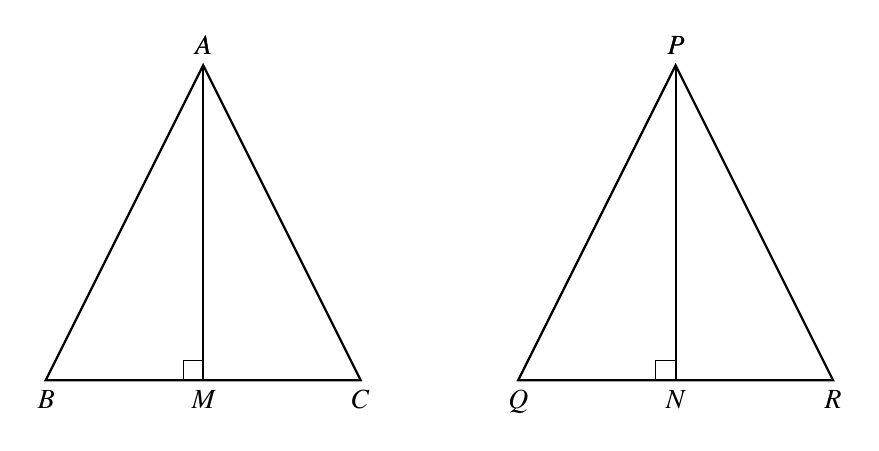
\begin{tikzpicture}
\coordinate (P) at (8,4);
\coordinate (Q) at (6,0);
\coordinate (R) at (10,0);
\coordinate (N) at (8,0);
\coordinate (A) at (2,4);
\coordinate (B) at (0,0);
\coordinate (C) at (4,0);
\coordinate (M) at (2,0);
\draw [black, thick](A)node[above]{$A$}--(B)node[below]{$B$}--(C)node[below]{$C$}--cycle;
\draw[black, thick] (P)node[above]{$P$}--(Q)node[below]{$Q$}--(R)node[below]{$R$}--cycle;
\draw[black, thick](M)node[below]{$M$}--(A)node[above]{$A$};
\draw[black, thick](N)node[below]{$N$}--(P)node[above]{$P$};
\tkzMarkRightAngle(A,M,B)
\tkzMarkRightAngle(P,N,Q)
\end{tikzpicture}}
	\caption{\triangle ABC and \triangle PQR}
	\label{myfig}
\end{figure}
Given Condition in the question are:
\begin{align}
&AB = PQ\label{eq1} \\
&BC = QR\label{eq2} \\
&AM = PN\label{eq3}
\end{align}
As M and N are medians of triangle ABC and triangle PQR respectively, we deduce the following:
\begin{align}
&\vec{M} = \frac{\vec{B}+\vec{C}}{2} \\
&\implies 2\vec{M} = \brak{\vec{B+C}}\\
&\implies\brak{\vec{B-M}} = \brak{\vec{M-C}}\\
&\implies\norm{\vec{B}-\vec{M}}=\norm{\vec{M}-\vec{C}}\label{eq5} \\
\text{Also}\\
&\vec{N} = \frac{\vec{Q}+\vec{R}}{2}\label{eq6} \\
&\implies2\vec{N} = \brak{\vec{Q+R}}\\
&\implies\brak{\vec{Q-N}} = \brak{\vec{N-R}}\\
&\implies\norm{\vec{Q}-\vec{N}}=\norm{\vec{N}-\vec{R}}\label{eq7}
\end{align}
Refer\eqref{eq5}and \eqref{eq7}
\begin{align}
&\norm{\vec{B}-\vec{M}}= \norm{\vec{Q}-\vec{N}}
\end{align}
Hence in triangle ABM and triangle PQN sides AB,BM and MA are equal to PQ,QN and NP so by SSS congruency criteria 
\begin{align}
    \triangle{ABM}\cong\triangle{PQN}\label{eqA}
\end{align}
Now for proving congruence of triangle ABC and triangle PQR we know that the corresponding angles of congurent triangles are equal and to prove that we make a hypothesis and proceed as follows
\begin{align}
\angle ABM = \angle PQN\label{eq8} 
\end{align} 
and one of the proved condition
\begin{align}
  BM=QN\label{eq9}  
\end{align}
Refer\eqref{eq8}\\
\begin{align}
\cos \angle ABM=\cos \angle PQN    
\end{align}
\begin{align}
\frac{\left( \vec{ B - A} \right)^T  \left( \vec{B - M } \right)}{\norm{\vec{ B - A}} \norm{\vec{B - M}}}=\frac{\left( \vec{ Q - P} \right)^T  \left( \vec{Q - N} \right)}{\norm{\vec{ Q - P}} \norm{\vec{Q - N}}}
\end{align}
Equating \eqref{eq9}
\begin{multline}
\label {eq10} 
\implies\frac{\left( \vec{ B - A} \right)^T  \left( \vec{B - M} \right)}{\norm{\vec{ B - A}}}=\\
\frac{\left( \vec{ Q - P} \right)^T  \left( \vec{Q - N } \right)}{\norm{\vec{ Q - P}}}
\end{multline}
It can be shown that
\begin{multline}
\label{eq11}
 \left( \vec{ B - A} \right)^T  \left( \vec{B - M} \right)=\\
 \norm{\vec{A - B}}^2 - \left ( \vec{  A - M  }\right)^T \left( \vec{A - B} \right)
 \end{multline}
 \begin{multline}
 \label{eq12}
 \left( \vec{ Q - P} \right)^T  \left( \vec{ Q- N } \right)=\\
 \norm{\vec{P - Q}}^2 - \left ( \vec{  P - N  }\right)^T \left( \vec{P - Q} \right)
\end{multline}
Substituting \eqref{eq11} and \eqref{eq12} in \eqref{eq10}
\begin{multline}
\norm{\vec{A - B}}- \frac{\left( \vec{ A - M} \right)^T \left( \vec{A - B} \right)}{\norm{\vec{ B - A}}} =\\ \norm{\vec{P - Q}}- \frac{\left( \vec{ P - N} \right)^T \left( \vec{P- Q} \right)}{\norm{\vec{ Q - P}}}
\end{multline}
\begin{multline}
\norm{\vec{A - B}}- \norm{\vec{A - M}}\cos\angle BAM =\\  \norm{\vec{P - Q}}- \norm{\vec{P - N}}\cos\angle QPN   
\end{multline}
 Refer \eqref{eq1} and \eqref{eq3}
\begin{align}
\norm{\vec{A - B}}= \norm{\vec{P - Q}}
\end{align}
\begin{align}
\norm{\vec{A - M}}= \norm{\vec{P - N}}
\end{align}
\begin{align}
\therefore \cos\angle BAM =  \cos\angle QPN
\end{align}
\begin{align}
\implies \angle BAM = \angle QPN
\end{align}
Hence our hypothesis is right as we prove that corresponding angles of congurent triangles are equal. So we get 
\begin{align}
\angle ABM=\angle PQN    
\end{align}
\begin{align}
\therefore \angle ABC=\angle PQR    
\end{align}
So by applying SAS criteria we conclude that\\
\begin{align}
\triangle{ABC}\cong\triangle{PQR}
\end{align}
\end{document}
